%%%%%%%%%%%%%%%%%%%%%%%%%%%%%%%%%%%%%%%%%%%%%%%%%%%%%%%%%%%%%%%%%%%%%%%%%%%%%%%%
%% Project: Fanclub Mark II %% File: fcmkii_document.tex                      %%
%%----------------------------------------------------------------------------%%
%% CALIFORNIA INSTITUTE OF TECHNOLOGY %% GRADUATE AEROSPACE LABORATORY %%     %%
%% CENTER FOR AUTONOMOUS SYSTEMS AND TECHNOLOGIES                             %%
%%----------------------------------------------------------------------------%%
%%      ____      __      __  __      _____      __      __    __    ____     %%
%%     / __/|   _/ /|    / / / /|  _- __ __\    / /|    / /|  / /|  / _  \    %%
%%    / /_ |/  / /  /|  /  // /|/ / /|__| _|   / /|    / /|  / /|/ /   --||   %%
%%   / __/|/ _/    /|/ /   / /|/ / /|    __   / /|    / /|  / /|/ / _  \|/    %%
%%  / /|_|/ /  /  /|/ / // //|/ / /|__- / /  / /___  / -|_ - /|/ /     /|     %%
%% /_/|/   /_/ /_/|/ /_/ /_/|/ |\ ___--|_|  /_____/| |-___-_|/  /____-/|/     %%
%% |_|/    |_|/|_|/  |_|/|_|/   \|___|-    |_____|/   |___|     |____|/       %%
%%                   _ _    _    ___   _  _      __   __                      %%
%%                  | | |  | |  | T_| | || |    |  | |  |                     %%
%%                  | _ |  |T|  |  |  |  _|      ||   ||                      %%
%%                  || || |_ _| |_|_| |_| _|    |__| |__|                     %%
%%                                                                            %%
%%----------------------------------------------------------------------------%%
%% Alejandro A. Stefan Zavala %% <alestefanz@hotmail.com> %%                  %%
%%%%%%%%%%%%%%%%%%%%%%%%%%%%%%%%%%%%%%%%%%%%%%%%%%%%%%%%%%%%%%%%%%%%%%%%%%%%%%%%


%% DOCUMENT SETUP %%%%%%%%%%%%%%%%%%%%%%%%%%%%%%%%%%%%%%%%%%%%%%%%%%%%%%%%%%%%%%
\documentclass{article}

% PACKAGES ---------------------------------------------------------------------
\usepackage{fullpage} % Margins
\usepackage{verbatimbox} % Center verbatim
\usepackage{hyperref} % Section references
\usepackage[english]{babel} % Set language
\usepackage{tikz} % Fun drawings
	\usetikzlibrary{shapes.geometric, arrows, fit, positioning}
\usepackage{everysel} % Modify typewriter font justification
\usepackage{float} % More options for figures (which are floats)
	\floatstyle{boxed}
	\restylefloat{figure}	

% COMMAND RENEWAL --------------------------------------------------------------
\renewcommand{\contentsname}{CONTENTS}
\renewcommand{\partname}{PART}
\renewcommand{\refname}{REFERENCES}
\renewcommand{\labelitemii}{-}
\renewcommand{\familydefault}{cmtt}
% Modify typewriter font justification:
% (See http://texblog.net/latex-archive/plaintex/full-justification-with-typewriter-font/)
\EverySelectfont{%
	\fontdimen2\font=0.4em% interword space
	\fontdimen3\font=0.2em% interword stretch
	\fontdimen4\font=0.1em% interword shrink
	\fontdimen7\font=0.1em% extra space
	\hyphenchar\font=`\-% to allow hyphenation
}

% SHORTHANDS FOR COMMON PHRASES ------------------------------------------------

							%%%%%%%%%%%%%%%%%%%%%%%%%%%%%%%%%%%%%%%%%%%%%%%%%%%%
\newcommand{\version}{0} % <<------- SET DOCUMENT VERSION HERE 
							%%%%%%%%%%%%%%%%%%%%%%%%%%%%%%%%%%%%%%%%%%%%%%%%%%%%
							
\newcommand{\fc}{FCMkII}
\newcommand{\Fc}{Fanclub MkII}
\newcommand{\Fcc}{Fanclub}
\newcommand{\Fawt}{Fan Array Wind Tunnel}
\newcommand{\Fawts}{Fan Array Wind Tunnels}
\newcommand{\N}{NUCLEO-F429ZI}


\setlength{\parindent}{0pt}
\setlength{\parskip}{1em}

% TIKZ SHAPES SETUP ------------------------------------------------------------

\tikzstyle{startstop} = [rectangle, rounded corners, minimum width=2em, minimum height=1.2em, text centered, text width = 5em, draw = black, very thick, font=\scriptsize]

\tikzstyle{decision} = [diamond, minimum width=7em, minimum height=1.4em, text centered, draw=black, very thick, inner sep=-1, font=\scriptsize]

\tikzstyle{process} = [rectangle, minimum width=3em, minimum height=1.5em, text centered, text width = 5em, draw = black, very thick,font=\scriptsize]

\tikzstyle{arrow} = [thick, ->, >=stealth]

\tikzstyle{message} = [dashed, thick, ->, >=stealth]


\tikzstyle{component} = [rectangle, minimum width=5em, minimum height=1.5em,  text width = 10em, draw = black, thick,font=\small]

\tikzstyle{subcomponent} = [rectangle, minimum width=3em, minimum height=1.5em, text centered, text width = 7em, draw = black,font=\scriptsize]


%% DOCUMENT %%%%%%%%%%%%%%%%%%%%%%%%%%%%%%%%%%%%%%%%%%%%%%%%%%%%%%%%%%%%%%%%%%%%
\begin{document}

%% TITLE PAGE ==================================================================
\begin{titlepage}

\vspace*{\fill}
\flushleft
\rule{\textwidth}{5pt}\\[1em]
\centering
\begin{minipage}{0.8\textwidth}
\begin{verbnobox}[\ttfamily\fontdimen2\font=5.24995pt\fontdimen3\font=0.0pt\fontdimen4\font=0.0pt\fontdimen7\font=5.24995pt\hyphenchar\font=-1]
	      ____      __      __  __      _____      __      __    __    ____     
     / __/|   _/ /|    / / / /|  _- __ __\    / /|    / /|  / /|  / _  \    
    / /_ |/  / /  /|  /  // /|/ / /|__| _|   / /|    / /|  / /|/ /   --||   
   / __/|/ _/    /|/ /   / /|/ / /|    __   / /|    / /|  / /|/ / _  \|/    
  / /|_|/ /  /  /|/ / // //|/ / /|__- / /  / /___  / -|_ - /|/ /     /|     
 /_/|/   /_/ /_/|/ /_/ /_/|/ |\ ___--|_|  /_____/| |-___-_|/  /____-/|/     
 |_|/    |_|/|_|/  |_|/|_|/   \|___|-    |_____|/   |___|     |____|/       
                     _ _    _    ___   _  _      __   __                      
                    | | |  | |  | T_| | || |    |  | |  |                     
                    | _ |  |T|  |  |  |  _|      ||   ||                      
                    || || |_ _| |_|_| |_| _|    |__| |__|                     
	
\end{verbnobox}
\end{minipage}

{\centering


}
\vspace{2em}
\texttt{\large "FANCLUB MkII" USER MANUAL AND DESIGN SPECIFICATION (\version)}\\
\texttt{\small Revised \today}

\rule{\linewidth}{5pt}

\vspace{5em}

\centering
\textsc{\Large Alejandro A. Stefan Zavala}\\
\textit{alestefanz@hotmail.com}
\vspace{5em}



\begin{minipage}{0.49\textwidth}
	\begin{flushleft}
		\textsc{\underline{Institution:}}\\
		California Institute of Technology\\
		Graduate Aerospace Laboratory \&\\
		Center for Autonomous Systems and Technologies\\
		1200 East California Boulevard\\
		Pasadena, California 91125\\
	\end{flushleft}
\end{minipage}
\hfill
\begin{minipage}{0.49\textwidth}
	\begin{flushright}
		\textsc{\underline{Supervisors:}}\\
		\vspace{1em}
		Christopher J. Dougherty\\
		\textit{cdougher@caltech.edu}\\
		Marcel Veismann\\
		\textit{mveisman@caltech.edu}
	\end{flushright}
\end{minipage}

\vspace*{\fill}

\end{titlepage}

%% TABLE OF CONTENTS ===========================================================
\begin{titlepage}
	\tableofcontents
\end{titlepage}

%% INTRODUCTION % % % % % % % % % % % % % % % % % % % % % % % % % % % % % % % % 
\section*{INTRODUCTION}
\addcontentsline{toc}{section}{INTRODUCTION}
[Leave the introduction for last!]
[In short, the purpose of the \Fcc project is the operation of \Fawts. More specifically... ]
\pagebreak

\section*{NAMING CONVENTIONS}
\addcontentsline{toc}{section}{NAMING CONVENTIONS}
[By the time I found out the correct spelling would be "Fan Club," it was too late.]

%% PART I: USER MANUAL % % % % % % % % % % % % % % % % % % % % % % % % % % % % %
\pagebreak
\part{USER MANUAL}


%% PART II: DESIGN SPECIFICATION % % % % % % % % % % % % % % % % % % % % % % % %
\pagebreak
\part{DESIGN SPECIFICATION}
\label{pDS}
Part II of this report describes the design process behind \Fc; this includes the underlying \hyperref[sec:Objs]{objectives}, \hyperref[sec:Pres]{precedents}, design choices made, and the reasoning behind them.

%% PRECEDENTS ==================================================================
\section{PRECEDENTS}
\label{sec:Pres}
[We stand on the shoulders of giants. We inherit the fruits of their greatness --- and the consequences of their sins.]\pagebreak

%% OBJECTIVES ==================================================================
\section{OBJECTIVES}
\label{sec:Objs}

\subsection{PRIMARY OBJECTIVES} % ----------------------------------------------
\label{ssec:PObjs}
These objectives\footnote{Additional requirements that are specific to communications can be found under \hyperref[sssec:ExpB]{EXPECTED BEHAVIOR}.} are critical to the use of \Fc\space and need be fulfilled. \fc \emph{ must}:

\begin{itemize}
	\item Given no ``external" failures (e.g misconfigured firewall, broken hardware), reliably secure a connection between the given Master and Slaves in the network (as chosen by the user), and, furthermore
	\begin{itemize}
		\item Maintain said connection until it is terminated either by the user or an external failure
		\item Detect any external failures and adjust accordingly, whether by automatically reconnecting or alerting the user
		\item In the event of an unexpected disconnection, affected Slaves with active fans must immediately shut down said fans. This is to say that \emph{no fan can be ``on" if it cannot be turned off by the user.}
	\end{itemize}
	
	\item Low level fan control (I/O)
	
	\item Feedback loop
	
	\item Master control
	
	\item Display feedback at Master
	
	\item Slave feedback by Slave
	
	\item Detect bad fans
	
\end{itemize}

\subsection{SECONDARY OBJECTIVES} % --------------------------------------------
\label{ssec:SObjs}
These objectives are not critical to the use of \Fc\space, but are a significant enough improvement on the usefulness of the software to be pursued. Unlike the aforementioned objectives, failure to meet any of these objectives does not render the software unfit for its mission. \fc\space may:

\begin{itemize}
	\item GUI
	
	\item Graphing
	
	\item All parameters
	
	\item Save profiles and logs
	
	\item Graph measurements
	
\end{itemize}

\subsection{ADDITIONAL OBJECTIVES} % -------------------------------------------
\label{ssec:AObjs}
Lastly, although these objectives are not pursued in the current design, they are worth documenting as potential for future work.
\begin{itemize}
	\item ``Offline" full-tunnel operation, possibly w/ LCD
	
	\item USB mode
	
	\item ``Online" software loading onto Slaves
	
\end{itemize}

\pagebreak

%% GENERAL =====================================================================
\section{GENERAL SPECIFICATION}
\label{sec:Gspe}

\subsection{GENERAL NETWORKING} % ----------------------------------------------
\label{sec:Gnet}

One of the defining tasks of \Fc\space is that of conveying information from the user to the system's microcontroller units (commands...) and vice versa (replies, measurements...). This is achieved through networking --- in particular, this is achieved using low-level socket programming in a form of [...]

\subsubsection{EXPECTED BEHAVIOR}
\label{sssec:ExpB}
The networking capability of \Fc\space must satisfy the following:

\begin{itemize}
	
	\item Both Master and Slaves can handle irresponsiveness from the other party, by verifyin the connection, attempting reconnection, or issuing disconnection alerts.
	
	\item Slaves can detect "irresponsive" networks --- defined here as one in which no IP address can be obtained using the Mbed \textit{EthernetInterface} class, which in most cases implies the Slave is physically disconnected. Furthermore:
	
	\begin{itemize}
		\item Slaves in such irresponsive networks will automatically resume normal execution when the network is fixed, without the need to be restarted by the user, no matter at what point of execution the network becomes irresponsive.
	\end{itemize}

	\item Once a connection is established, the user will receive (in Master) periodic updates on the state of the connected Slaves without the need for explicit request. These updates include the current task, if any, and most recent RPM reading of all active fans; the period of these updates can be configured, but is expected to be of less than a second.
	
	\item The "relevant" information of a Slave can be accessed (and modified, if applicable) through Master once a connection is established. The information deemed "relevant" is defined in [\#\&SLAVE PROFILE].
	
\end{itemize}


\subsubsection{SUMMARY}

The flow chart below summarizes the communications process between Master and Slave. Note that this is a simplified illustration of the actual algorithm.

\begin{figure}[h]
\begin{center}
\vspace{1em}
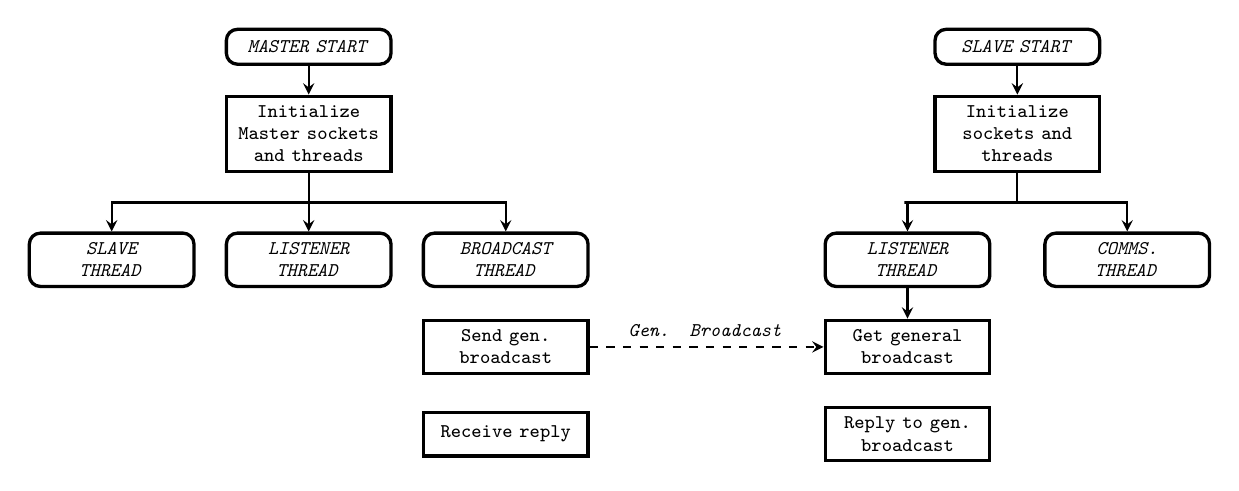
\begin{tikzpicture}[node distance = 3em]

	% Master nodes - - - - - - - - - - - - - - - - - - - - - - - - - - - - - - -
	
	%MASTER START
	\node(mstart) [startstop]{\textit{MASTER START}};
	%Initialize Master sockets and threads
	\node(minit) [process, below of= mstart]
		{Initialize Master sockets and threads
		};
	%MASTER BROADCAST THREAD . . . . . . . . . . . . . . . . . . . . . . . . . . 
	\node(minitb)[startstop, below right= 2em and 1em of minit] 
		{\textit{BROADCAST\\THREAD} };
		
		%Send broadcast
		\node(msendb)[process,below of=minitb]
			{Send gen. broadcast};
			
		%Receive reply
		\node(mgetb) [process, below of= msendb]
		{Receive reply
		};
		
		
	%MASTER LISTENER THREAD . . . . . . . . . . . . . . . . . . . . . . . . . . 
	\node(minitl)[startstop, below= 2em of minit] 
	{\textit{LISTENER\\THREAD} };
	
	% Slave nodes - - - - - - - - - - - - - - - - - - - - - - - - - - - - - - -
	\node(sstart)[startstop,right of = mstart, node distance = 9cm]{\textit{SLAVE START}};
	
	% Initialize sockets and threads
	\node(sinit) [process, below of= sstart]
	{Initialize sockets and threads
		};
	
	%MASTER SLAVE THREAD . . . . . . . . . . . . . . . . . . . . . . . . . . . .
	\node(minits)[startstop, below left= 2em and 1em of minit] 
	{\textit{SLAVE\\THREAD} };
	
	%SLAVE LISTENER THREAD . . . . . . . . . . . . . . . . . . . . . . . . . . .
	\node(sinitl)[startstop, below left= 2em and -2em of sinit] 
	{\textit{LISTENER\\THREAD} };
	
	\node(sgetb) [process, below of= sinitl]
		{Get general broadcast
		};
	
	\node(ssendb) [process, below of= sgetb]
		{Reply to gen. broadcast
		};
	
	%SLAVE COMMUNICATION THREAD . . . . . . . . . . . . . . . . . . . . . . . . 
	\node(sinitc)[startstop, below right= 2em and -2em of sinit] 
	{\textit{COMMS.\\THREAD} };

	% Master arrows - - - - - - - - - - - - - - - - - - - - - - - - - - - - - - 
	\draw[arrow](mstart)--(minit);
	\draw[arrow](minit)--(minitl);
	\draw[arrow](minit)|-([shift={(-1em,-1em)}]minit.south east)-|(minitb);
	\draw[arrow](minit)|-([shift={(-1em,-1em)}]minit.south west)-|(minits);
	\draw[message](msendb)--node[anchor = south]{\textit{\scriptsize Gen. Broadcast}}(sgetb);
	
	% Slave arrows - - - - - - - - - - - - - - - - - - - - - - - - - - - - - - -
	\draw[arrow](sstart)--(sinit);
	\draw[arrow](sinitl)--(sgetb);
	\draw[arrow](sinit)|-([shift={(-1em,-1em)}]sinit.south west)-|(sinitl);
	\draw[arrow](sinit)|-([shift={(-1em,-1em)}]sinit.south east)-|(sinitc);
	
\end{tikzpicture}
\end{center}
\caption{Illustrated summary of communications between Master and one Slave}
\end{figure}
\pagebreak


%% MASTER ======================================================================
\section{"MASTER" SPECIFICATION}
\label{sec:Mspe}



%% SLAVE =======================================================================
\section{"SLAVE" SPECIFICATION}
\label{sec:Sspe}

\subsection{MODULAR BREAKDOWN}
\label{sec:Mbre}

\begin{center}
\begin{figure}[h]
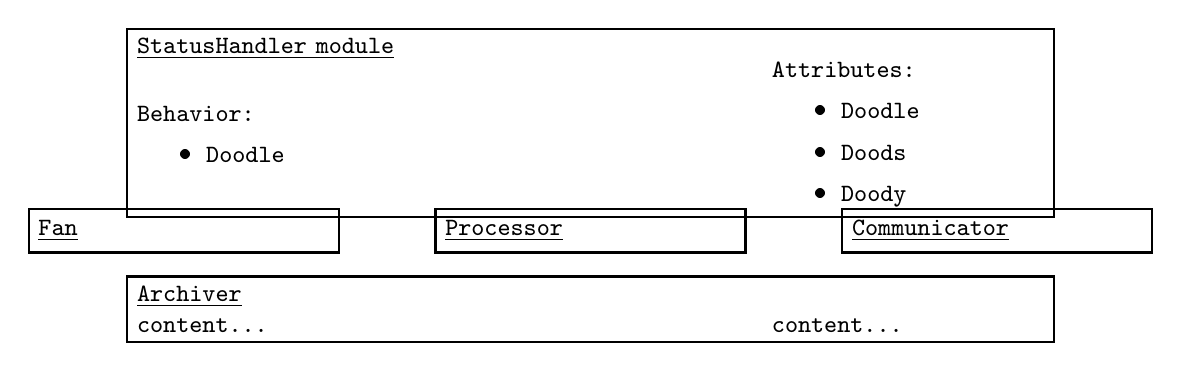
\begin{tikzpicture}

% StatusHandler module:
\node(status)[component, text width = 0.95\linewidth]
{\underline{StatusHandler module}\\
	\begin{minipage}{0.3\linewidth}
	Behavior:
		\begin{itemize}
		\item Doodle
		\end{itemize}
	\end{minipage}
	\hspace*{\fill}
	\begin{minipage}{0.3\linewidth}
	Attributes:
	\begin{itemize}
	\item Doodle
	\item Doods
	\item Doody
	\end{itemize}
	\end{minipage}
};

% Processor module:
\node(pross)[component, below of=status,yshift=-1em]
{\underline{Processor}};

% Communicator module:
\node(comms)[component, right of=pross, node distance = 14em]
{\underline{Communicator}};

% Fan module:
\node(fan)[component, left of=pross, node distance = 14em]
{\underline{Fan}};


% Archiver module"
\node(archiver)[component, text width = 0.95\linewidth, below of = pross]
{\underline{Archiver}\\
	\begin{minipage}{0.3\linewidth}
	content...
	\end{minipage}
	\hspace*{\fill}
	\begin{minipage}{0.3\linewidth}
	content...
	\end{minipage}
};



\end{tikzpicture}
\caption{Modular breakdown of the Slave program}
\end{figure}
\end{center}

\subsection{``SLAVE" NETWORKING} %% --------------------------------------------
\label{sec:sNspe}
	In a Slave, all networking functions (e.g receive a command, send a reply, secure a connection) are handled by its Communicator module.
	
%% REFERENCES % % % % % % % % % % % % % % % % % % % % % % % % % % % % % % % % % 
\pagebreak
\addcontentsline{toc}{section}{REFERENCES}
\begin{thebibliography}{5}
	
\end{thebibliography}


\end{document}